\documentclass{beamer}
\usepackage[utf8]{inputenc}
\usepackage[dutch]{babel}
\usepackage{hyperref}
% colored links
\hypersetup{
    colorlinks=true,
    linkcolor=blue,
    urlcolor=blue,
}
\usetheme{Madrid}
\usecolortheme{default}

%------------------------------------------------------------
%This block of code defines the information to appear in the
%Title page
\title[Debian installatie] %optional
{Debian installatie met preseed}

% \subtitle{A short story}

\author[S.L.Speek] % (optional)
{Steven L. Speek}

\institute[ACC] % (optional)
{
  Actief Computer Centrum
}

\date[\today{}] % (optional)
{\today{}}

% \logo{\includegraphics[height=1cm]{overleaf-logo}}

%End of title page configuration block
%------------------------------------------------------------



%------------------------------------------------------------
%The next block of commands puts the table of contents at the 
%beginning of each section and highlights the current section:

% \AtBeginSection[]
% {
%   \begin{frame}
%     \frametitle{Inhoudsopgave}
%     \tableofcontents[currentsection]
%   \end{frame}
% }
%------------------------------------------------------------


\begin{document}

%The next statement creates the title page.
\frame{\titlepage}


%---------------------------------------------------------
%This block of code is for the table of contents after
%the title page
\begin{frame}
\frametitle{Inhoudsopgave}
\tableofcontents
\end{frame}
%---------------------------------------------------------


\section{Installatie media}

%---------------------------------------------------------
\begin{frame}
\frametitle{Installatie media downloaden}
Klik `Downloaden' op \href{https://debian.org}{debian.org}

\centering
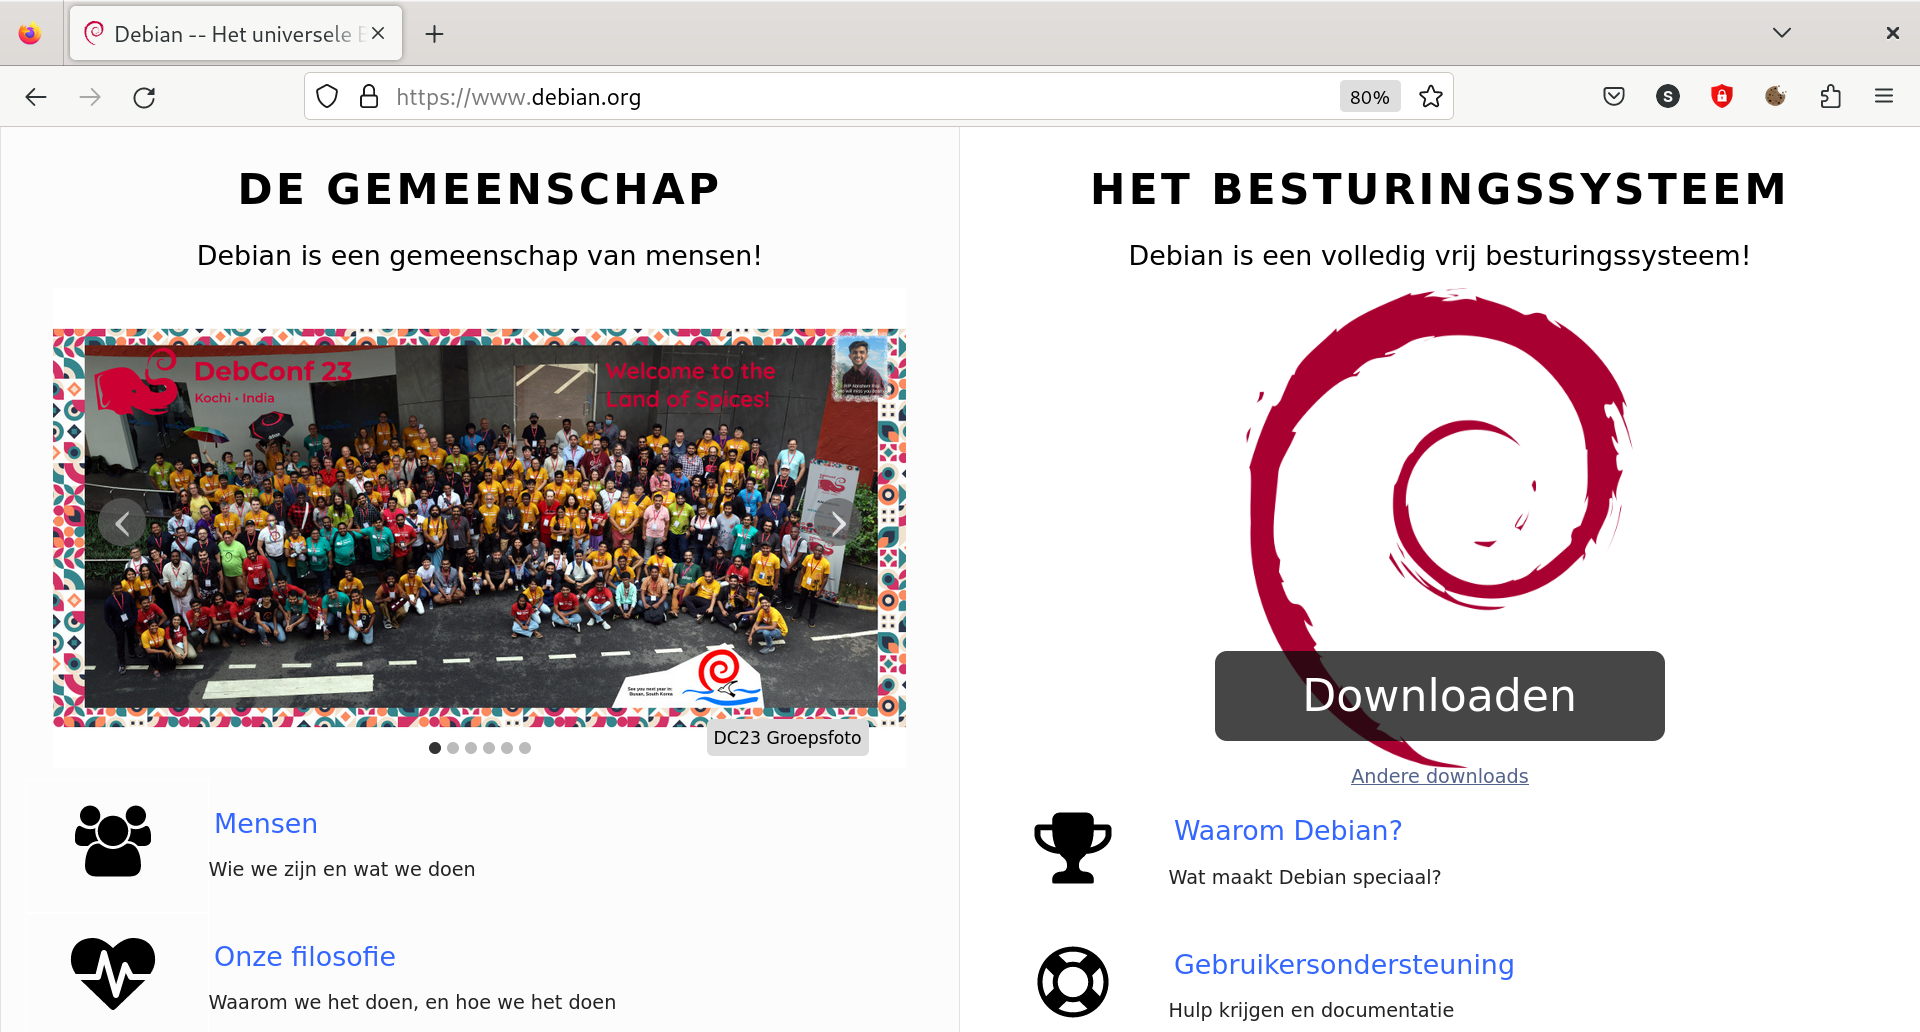
\includegraphics[width=\textwidth]{img/debian-downloaden.png} 
\end{frame}

\begin{frame}
  \frametitle{Installatie USB-stick maken}
\begin{itemize}
    \item Download en installeer \href{https://rufus.ie}{Rufus}
    \item Maak een USB-stick met het debian ISO-image met Rufus
\end{itemize}
\end{frame}

%---------------------------------------------------------


%---------------------------------------------------------
\section{De installer booten}

\begin{frame}
  \frametitle{De \textbf{debian-installer} booten}
  \begin{itemize}
    \item Steek de USB-stick met de debian ISO-image in de computer
    \item Start de computer op en ga het \href{https://www.boot-disk.com/quest_bootmenu.htm}{boot menu} in
  \end{itemize}

\end{frame}
%---------------------------------------------------------


%---------------------------------------------------------
\section{Automatische installatie}

\begin{frame}
  \frametitle{Geavanceerde installatie kiezen}

  \centering
  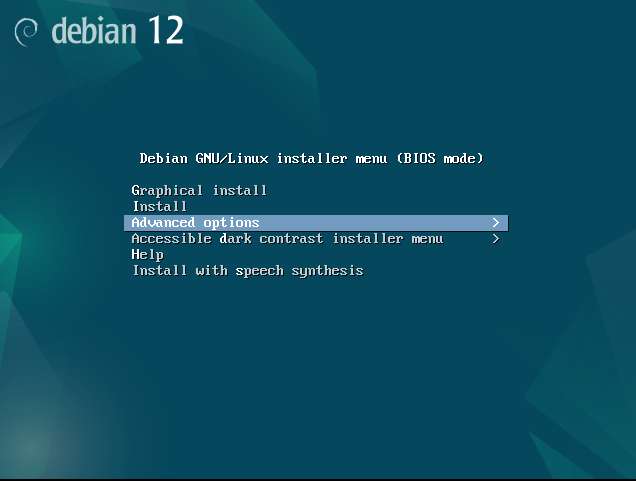
\includegraphics[width=\textwidth]{img/advanced-options.png}
\end{frame}

\begin{frame}
  \frametitle{Automatische installatie kiezen}

  \centering
  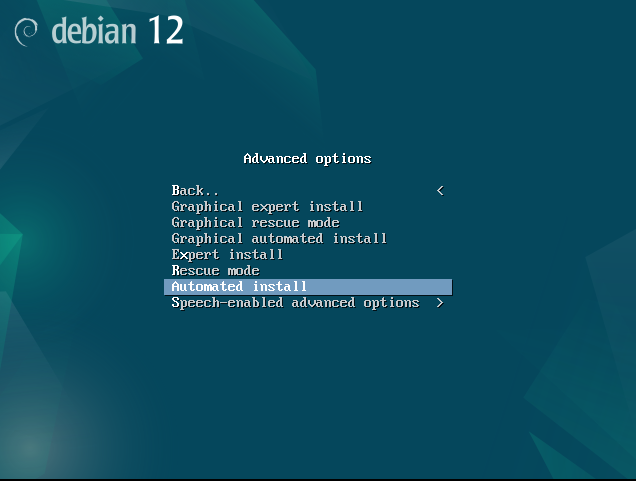
\includegraphics[width=\textwidth]{img/automated-install.png}
\end{frame}

%---------------------------------------------------------
%Two columns

\end{document}